\chapter{提案手法}
\label{proposed}

本章では提案手法について述べる.

\section{概要}

本研究では, 自動車の利用者である人間の状態と道路網を再現を再現するシミュレータープログラムを開発し, 自動車であるモビリティの経路選択を
DQNを用いて学習させた.
また, 道路網は計算量の問題などから全ての道を扱うことは困難であるから実在する道を参考に選び出し, 仮装の道路網を設定した.
なお, 本実験での環境シミュレーターは以下の条件で作成を行った.



\section{本実験における前提}

本実験では道路交通網をソフトウェアプログラムにより擬似的に再現する. その際に、実験を短略化させ結果が発生する要因を掴みやすくするため以下の条件を適用する.


\begin{itemize}
    \item 自動車は1区間を全て等速で動くものとする
    \item 事故や災害などによる道路の不通などアクシデントは一切想定しない
    \item 人間の状態は予め作成されたユースケースのみを想定する
    \item 全ての道路は上下線, 双方向での通行が可能なものとする
    \item 信号による制御などは考えないものとする.
\end{itemize}


\section{道路網の正規化}

本研究では実際の道路網を参考に仮想の道路網モデルを構築した.
選び出したルートの正則化を行った。実際の地図上にある道路のPOLYLINEデータは道路路線上の点の集合体であり, これを結んだ線分として記録されている. しかし, DQN機械学習モデルでは限られた次元数の行列データしか扱うことができず, そのままではDQNに学習させることができない。
そこで、本研究では、1つのPOLYLINEを交差点毎に分解し交差点に挟まれた1区間を行列の1次元に表し1つの要素とした.
この場合, 区間の距離に関わらず1次元の要素として表すため距離情報が失われる. 従って, ここでは距離を通過難易度dとして環境定義することで距離データを失わないようにした.

以下に, 道路の正規化の手順を示す.

\subsection{道路データのベクタライズアルゴリズム}

図~\ref{rs:1}は実際の地図から本研究で取り上げる道路網を線で表したものである. 赤色の線は一度に通行できるcapacityが多い幹線道路としオレンジは赤色と比べて通行可能量が少ない.

次に, 図~\ref{rs:2}は道路のT字路や十字路などの交差点の形は問わず交差点部分に青い円形のマークをつけた. 

図~\ref{rs:3}は図~\ref{rs:2}から背景となる実際の地図を消去したものである. ここまでは, 地図から手動でデータを作成した. このデータからDQNの学習に適したデータ形式へと作成したプログラムを用いて変換する.

図~\ref{rs:4}は図~\ref{rs:3}を直線化させ四角形に近似した物である. これは道路網を多次元配列で表現するための前処理である. なお, この処理を行った時点で道路本来の距離データが失われる.

図~\ref{rs:5}は図~\ref{rs:4}の交差点と交差点の間を1区間とした時, 頂点全てが交差点となる四角形が正方形になるように変換した物である. これにより道路網は正方行列で表現が可能となる.

図~\ref{rs:6}は~\ref{rs:5}似て変換された図形データを正方行列データに変換した物である. ここでは, 通行可能な要素を1とし通行不可能な壁0で隔てることにより道路網を表現している.
なお, 道路外周に壁を作るために0パディングを行っている.

本提案手法で想定されている道路形状は以下の通りである.


\begin{figure}[htbp]
    \begin{minipage}{0.5\hsize}
        \begin{center}
            \includegraphics[width=70mm]{assets/MAP_1.eps}
        \end{center}
        \caption{地図から道路を選択}
        \label{rs:1}
    \end{minipage}
    \begin{minipage}{0.5\hsize}
        \begin{center}
            \includegraphics[width=70mm]{assets/MAP_2.eps}
        \end{center}
        \caption{交差点をマーク}
        \label{rs:2}
    \end{minipage}
\end{figure}



\begin{figure}[htbp]
    \begin{minipage}{0.5\hsize}
        \begin{center}
            \includegraphics[width=70mm]{assets/MAP_3.eps}
        \end{center}
        \caption{地図を除いた道路図と交差点マーク}
        \label{rs:3}
    \end{minipage}
    \begin{minipage}{0.5\hsize}
        \begin{center}
            \includegraphics[width=70mm]{assets/MAP_4.eps}
        \end{center}
        \caption{曲線を直線化}
        \label{rs:4}
    \end{minipage}
\end{figure}




\begin{figure}[htbp]
    \begin{minipage}{0.5\hsize}
        \begin{center}
            \includegraphics[width=70mm]{assets/MAP_5.eps}
        \end{center}
        \caption{区間の長さを等しく正方形にする}
        \label{rs:5}
    \end{minipage}
    \begin{minipage}{0.5\hsize}
        \begin{center}
            \includegraphics[width=70mm]{assets/MAP_6.eps}
        \end{center}
        \caption{7x7正方行列化した道路網}
        \label{rs:6}
    \end{minipage}
\end{figure}




\subsection{想定した道路線形}

本研究で考案した道路データのベクタライズアルゴリズムに関しては, 以下の道路線形を想定した.
以下に順を追って説明する.

~\ref{Y}から~\ref{GradeSeparation}は道と交差・分岐点を表した模式図である. 赤色の線は道路を表し, 青い円は交差・分岐点を示す. なお立体交差地点のみ交差する線をそれぞれ異なる色で表している.

~\ref{Y}はY字分岐である. この線形は1本の道から2本の道へと分岐を表す.
~\ref{Merge}は合流点を表す. これは2本の道が合流し1本の道へとなる事を意味する.
~\ref{RightCorner}は右折点を表す. これは2本の道が右方向へと右折する.
また, ~\ref{LeftCorner}も同様に左折点を表す.
~\ref{T}はT字路を表す.
~\ref{Cross}は十字路を表し2本の線が交差し4方向に別れる道を想定している.
~\ref{RouteEnd}は行き止まり地点を表しこれ以上行く事はできない. 本研究においては, エージェントはここを目的地とした場合以外では選択してはならない道である.
~\ref{GradeSeparation}は立体交差構造である. 立体交差構造は上空からみた場合, 2本の線が交差し十字路と同じ形になるが, 実際には右左折する事は不可能である.



\begin{figure}[htbp]
    \begin{minipage}{0.5\hsize}
        \begin{center}
            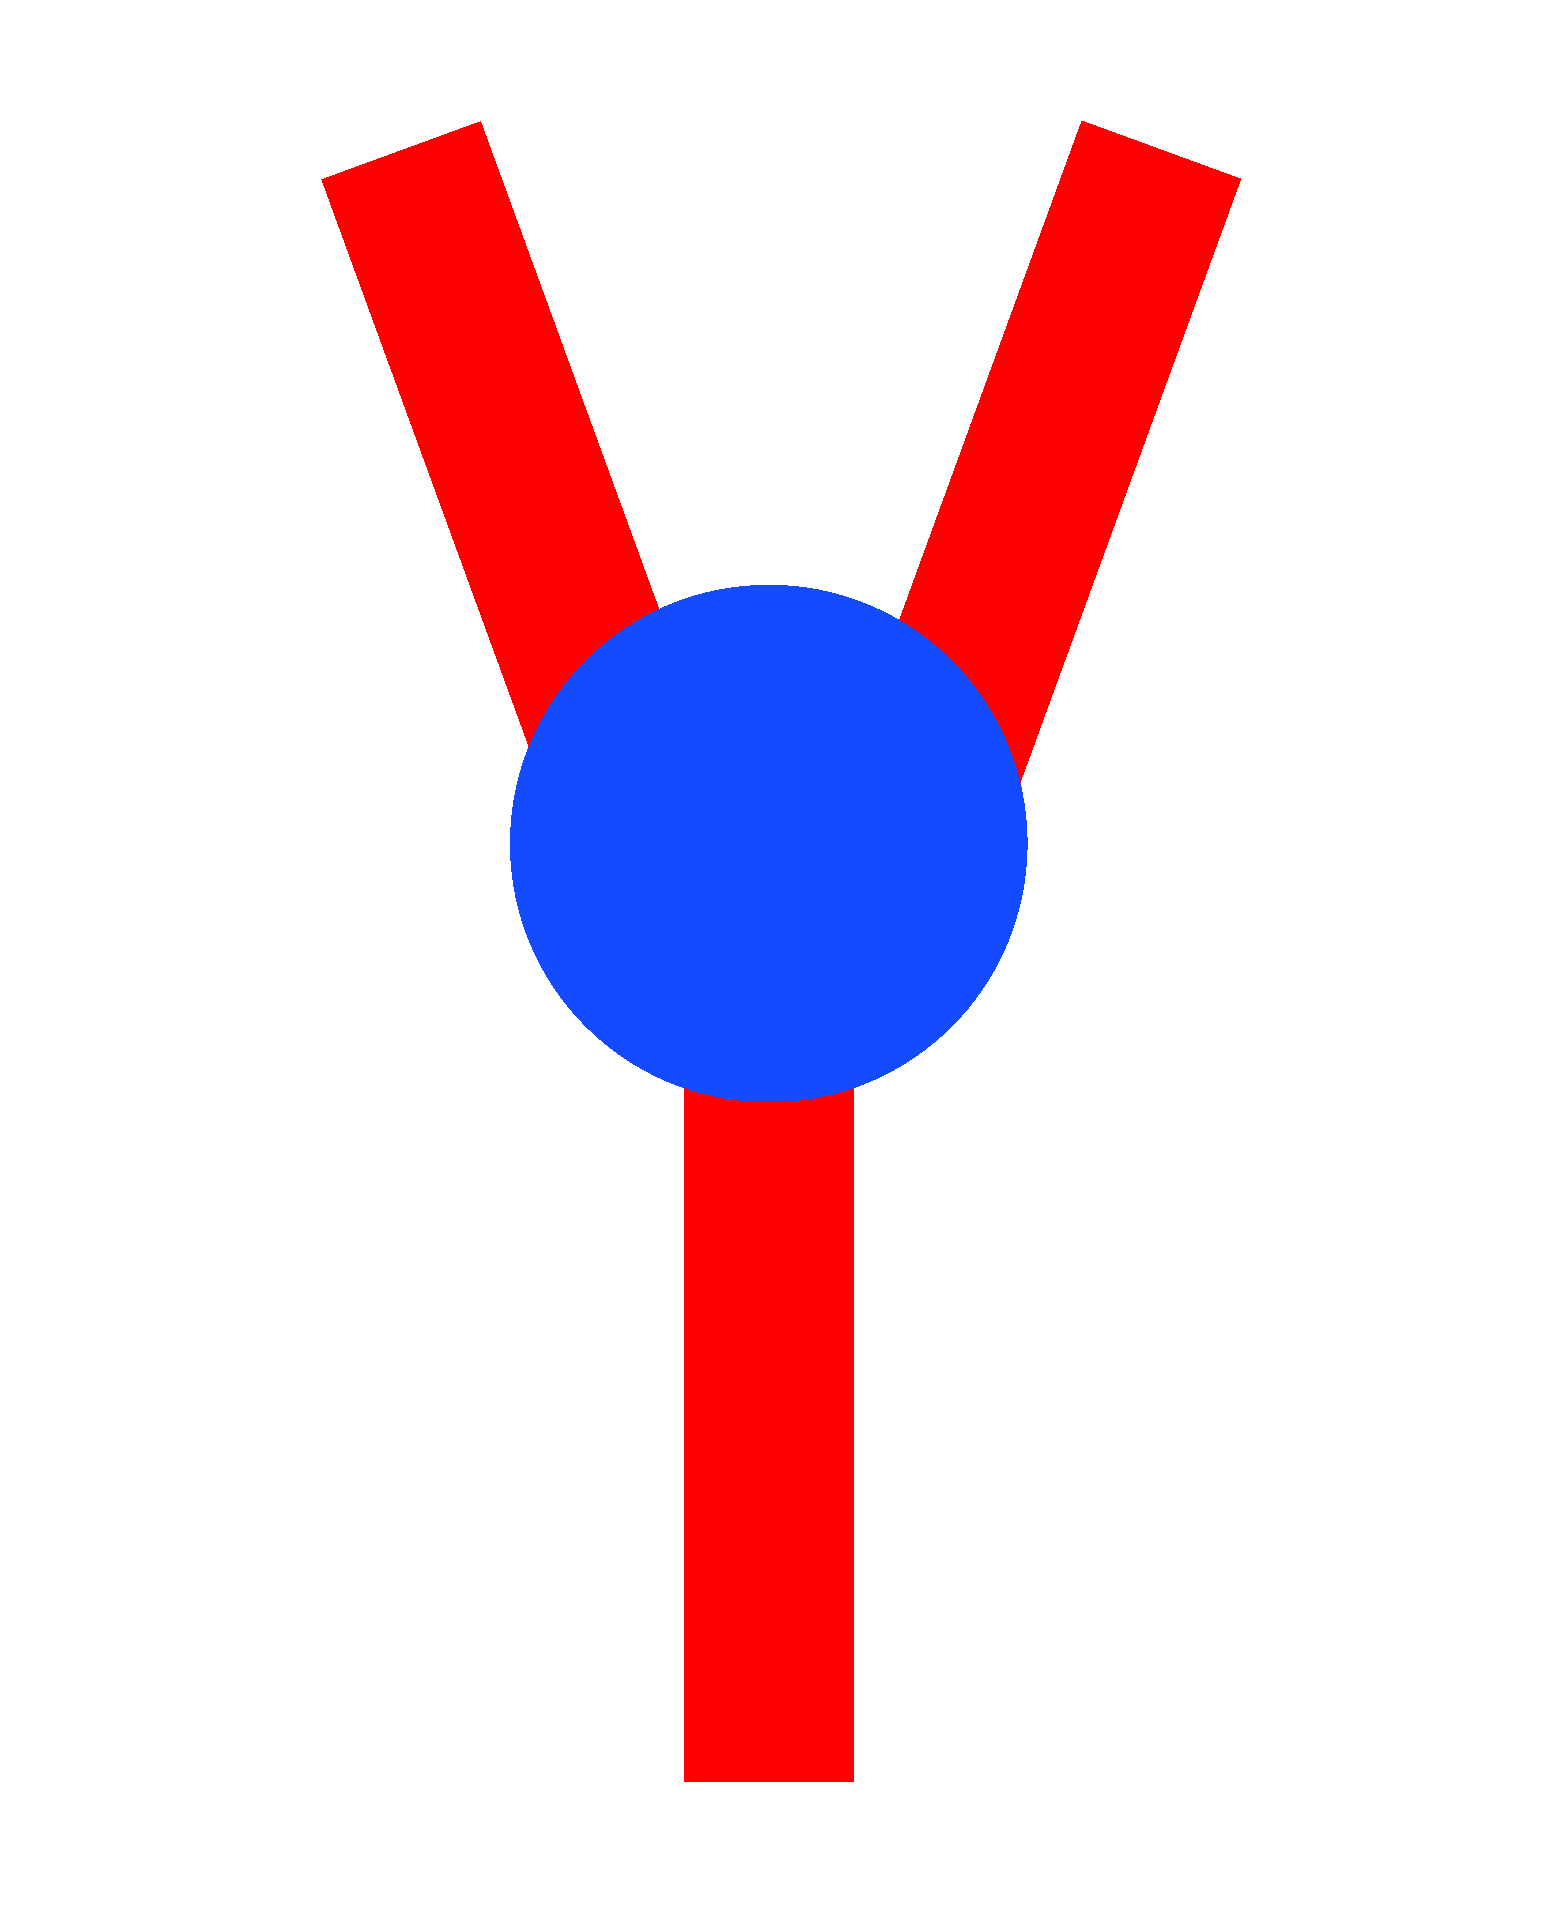
\includegraphics[,height=50mm]{assets/road_shape_Y.eps}
        \end{center}
        \caption{分岐}
        \label{Y}
    \end{minipage}
    \begin{minipage}{0.5\hsize}
        \begin{center}
            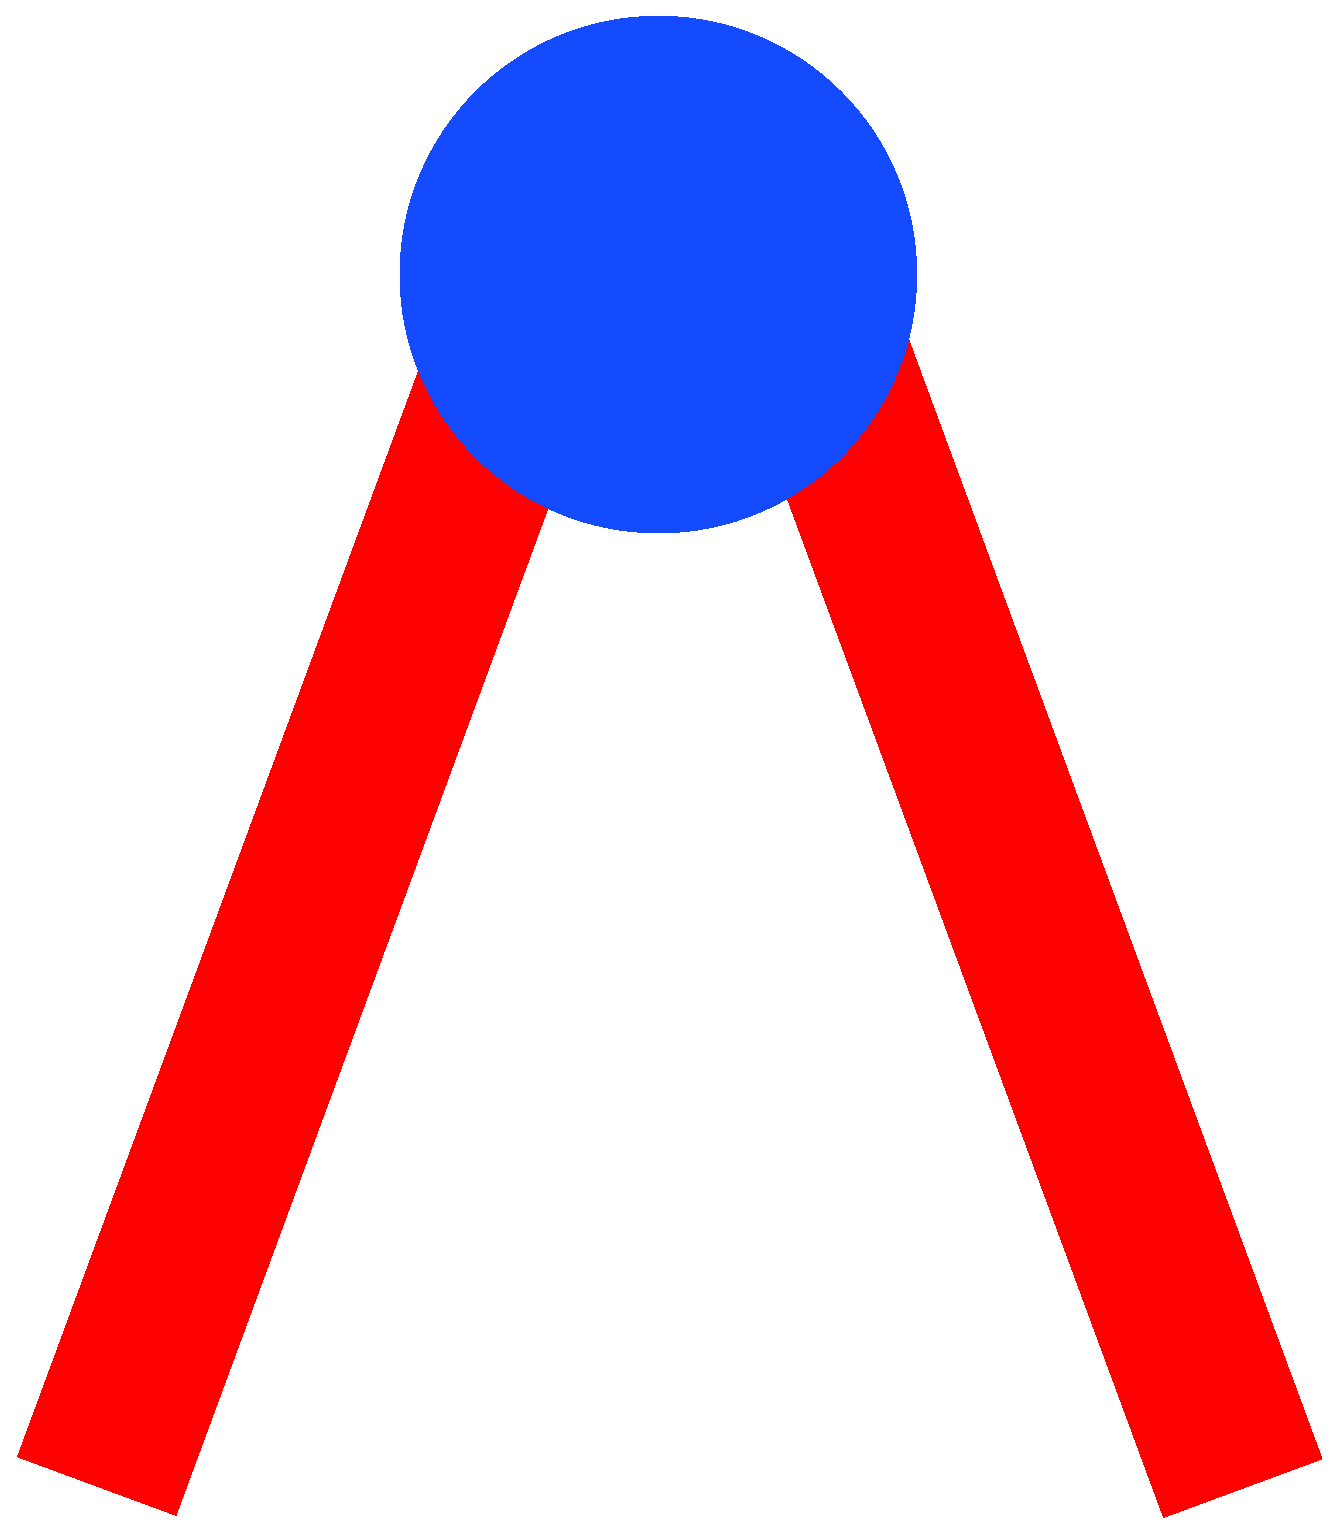
\includegraphics[,height=50mm]{assets/road_shape_Merge.eps}
        \end{center}
        \caption{合流}
        \label{Merge}
    \end{minipage}
\end{figure}




\begin{figure}[htbp]
    \begin{minipage}{0.5\hsize}
        \begin{center}
            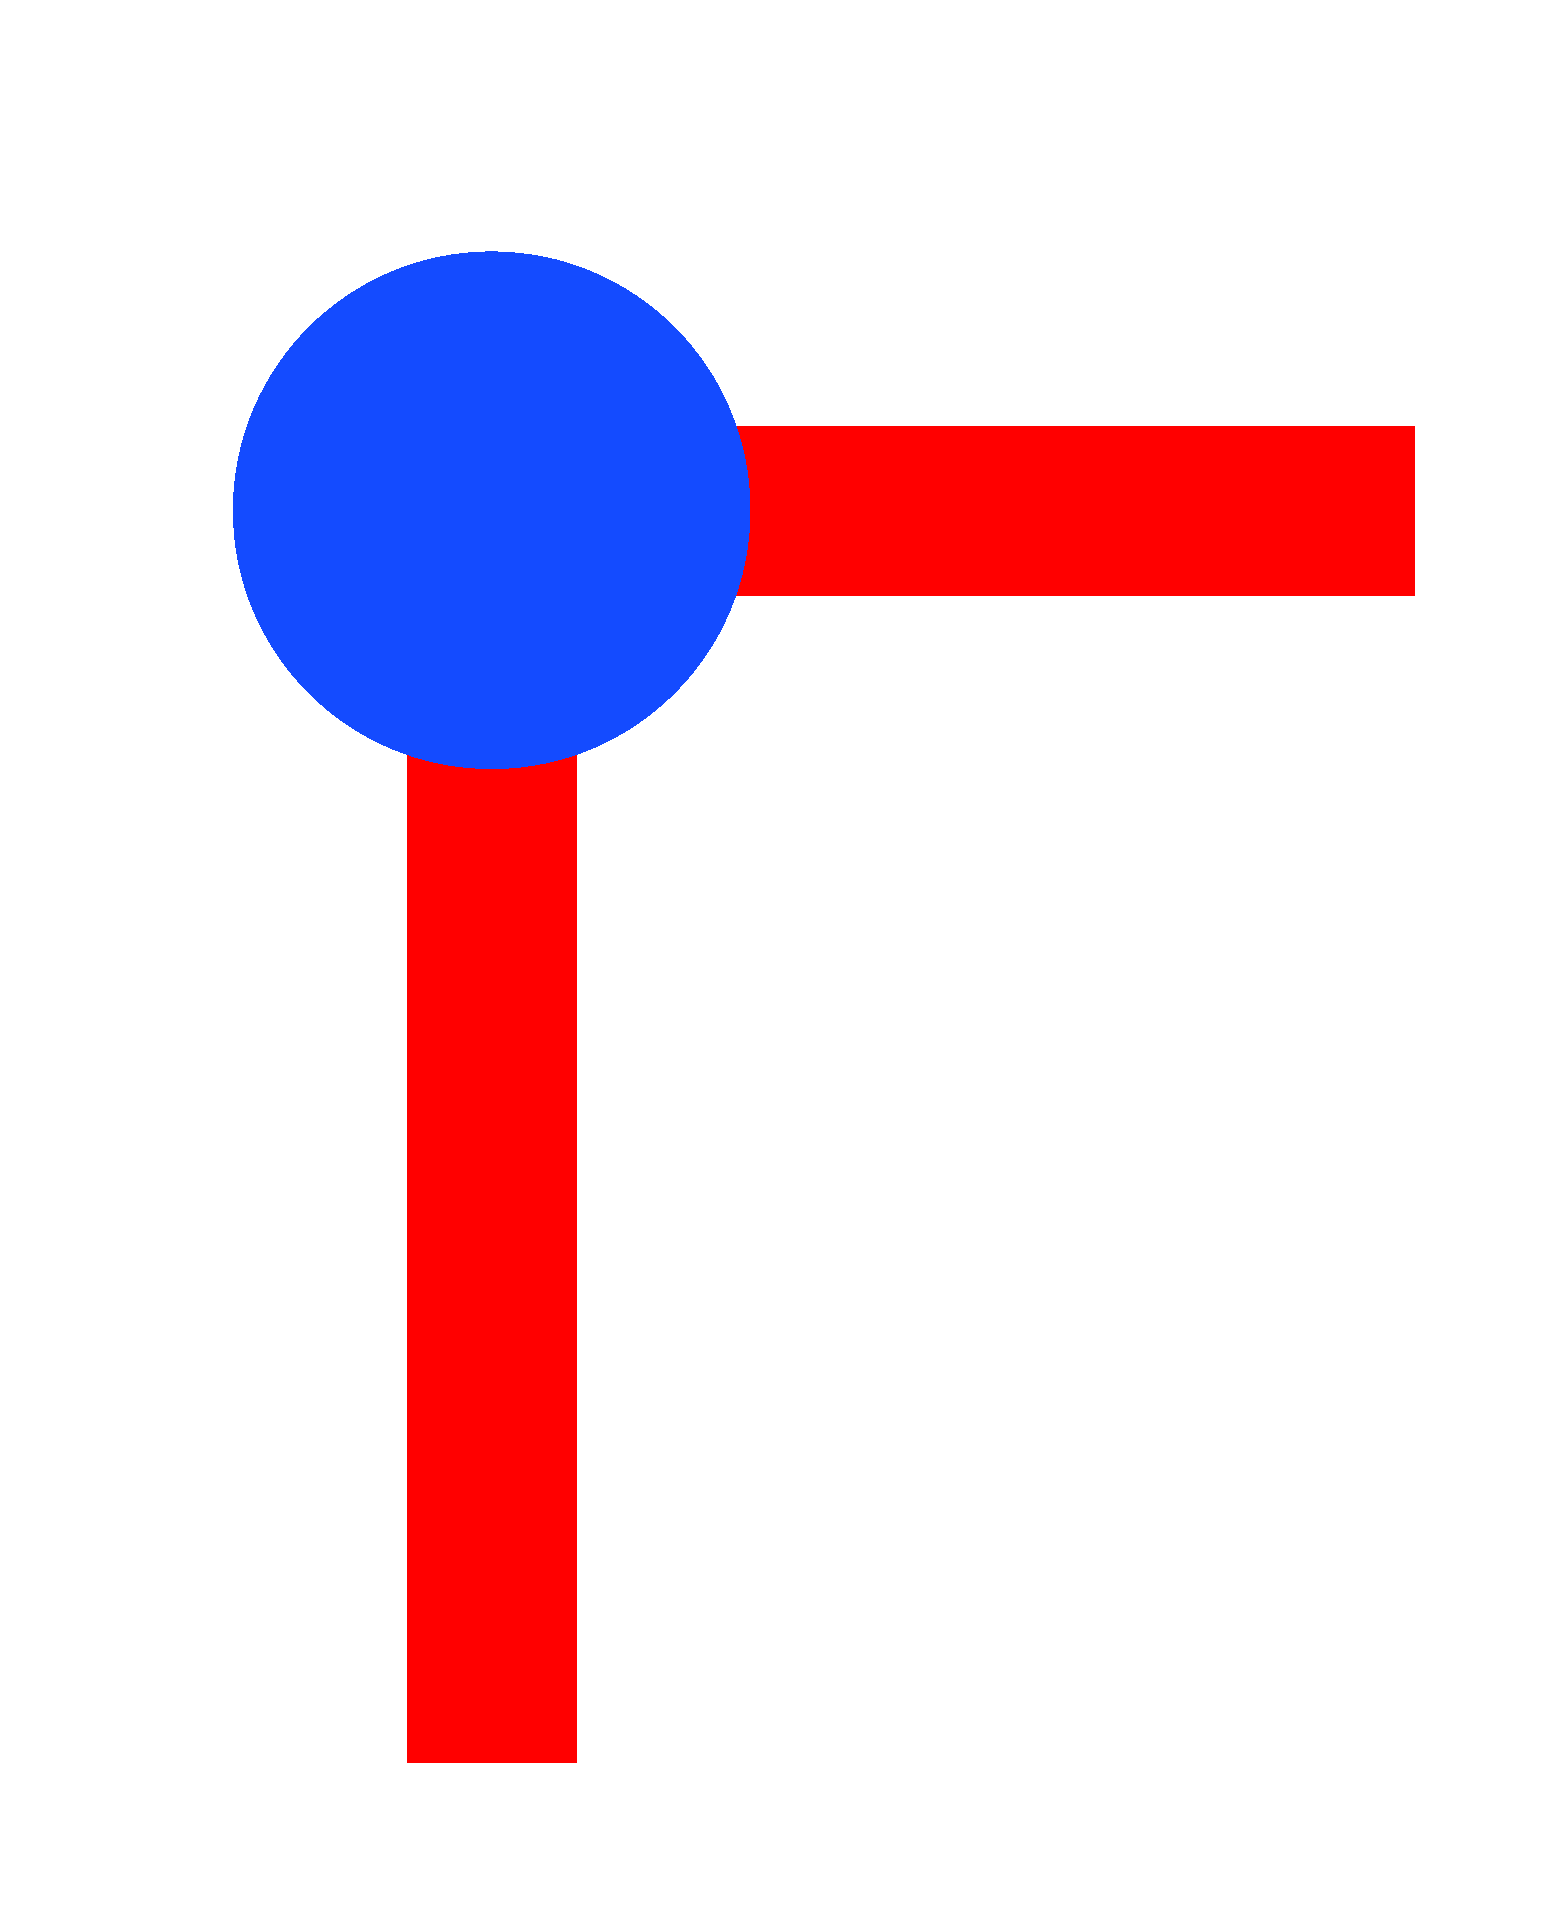
\includegraphics[,height=50mm]{assets/road_shape_RightCorner.eps}
        \end{center}
        \caption{右折}
        \label{RightCorner}
    \end{minipage}
    \begin{minipage}{0.5\hsize}
        \begin{center}
            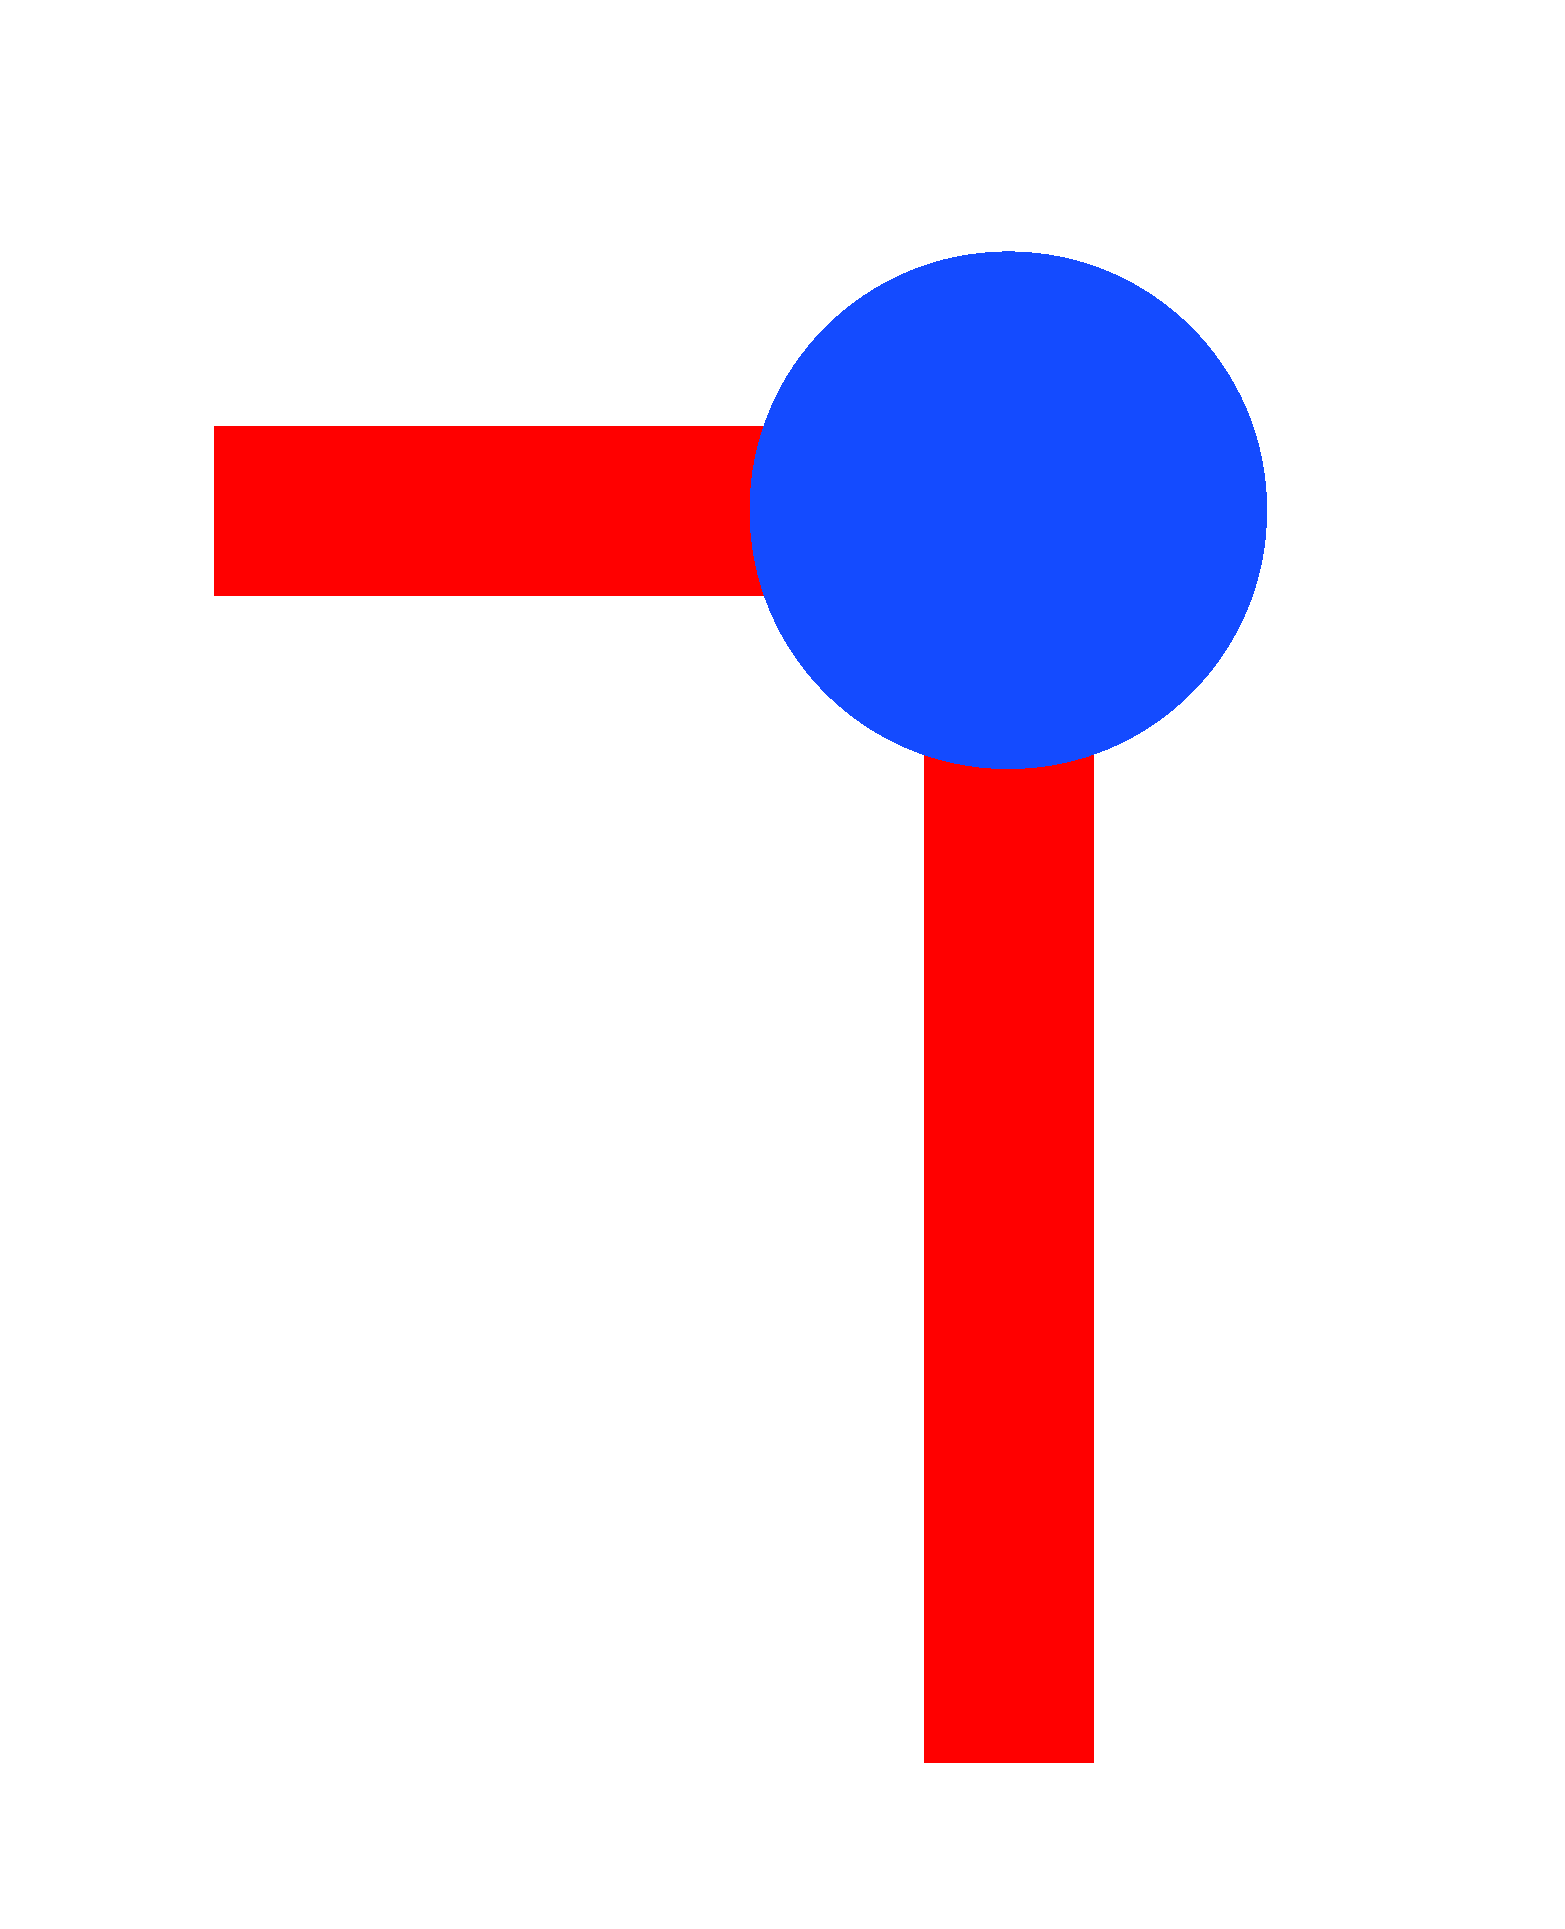
\includegraphics[,height=50mm]{assets/road_shape_LeftCorner.eps}
        \end{center}
        \caption{左折}
        \label{LeftCorner}
    \end{minipage}
\end{figure}



\begin{figure}[htbp]
    \begin{minipage}{0.5\hsize}
        \begin{center}
            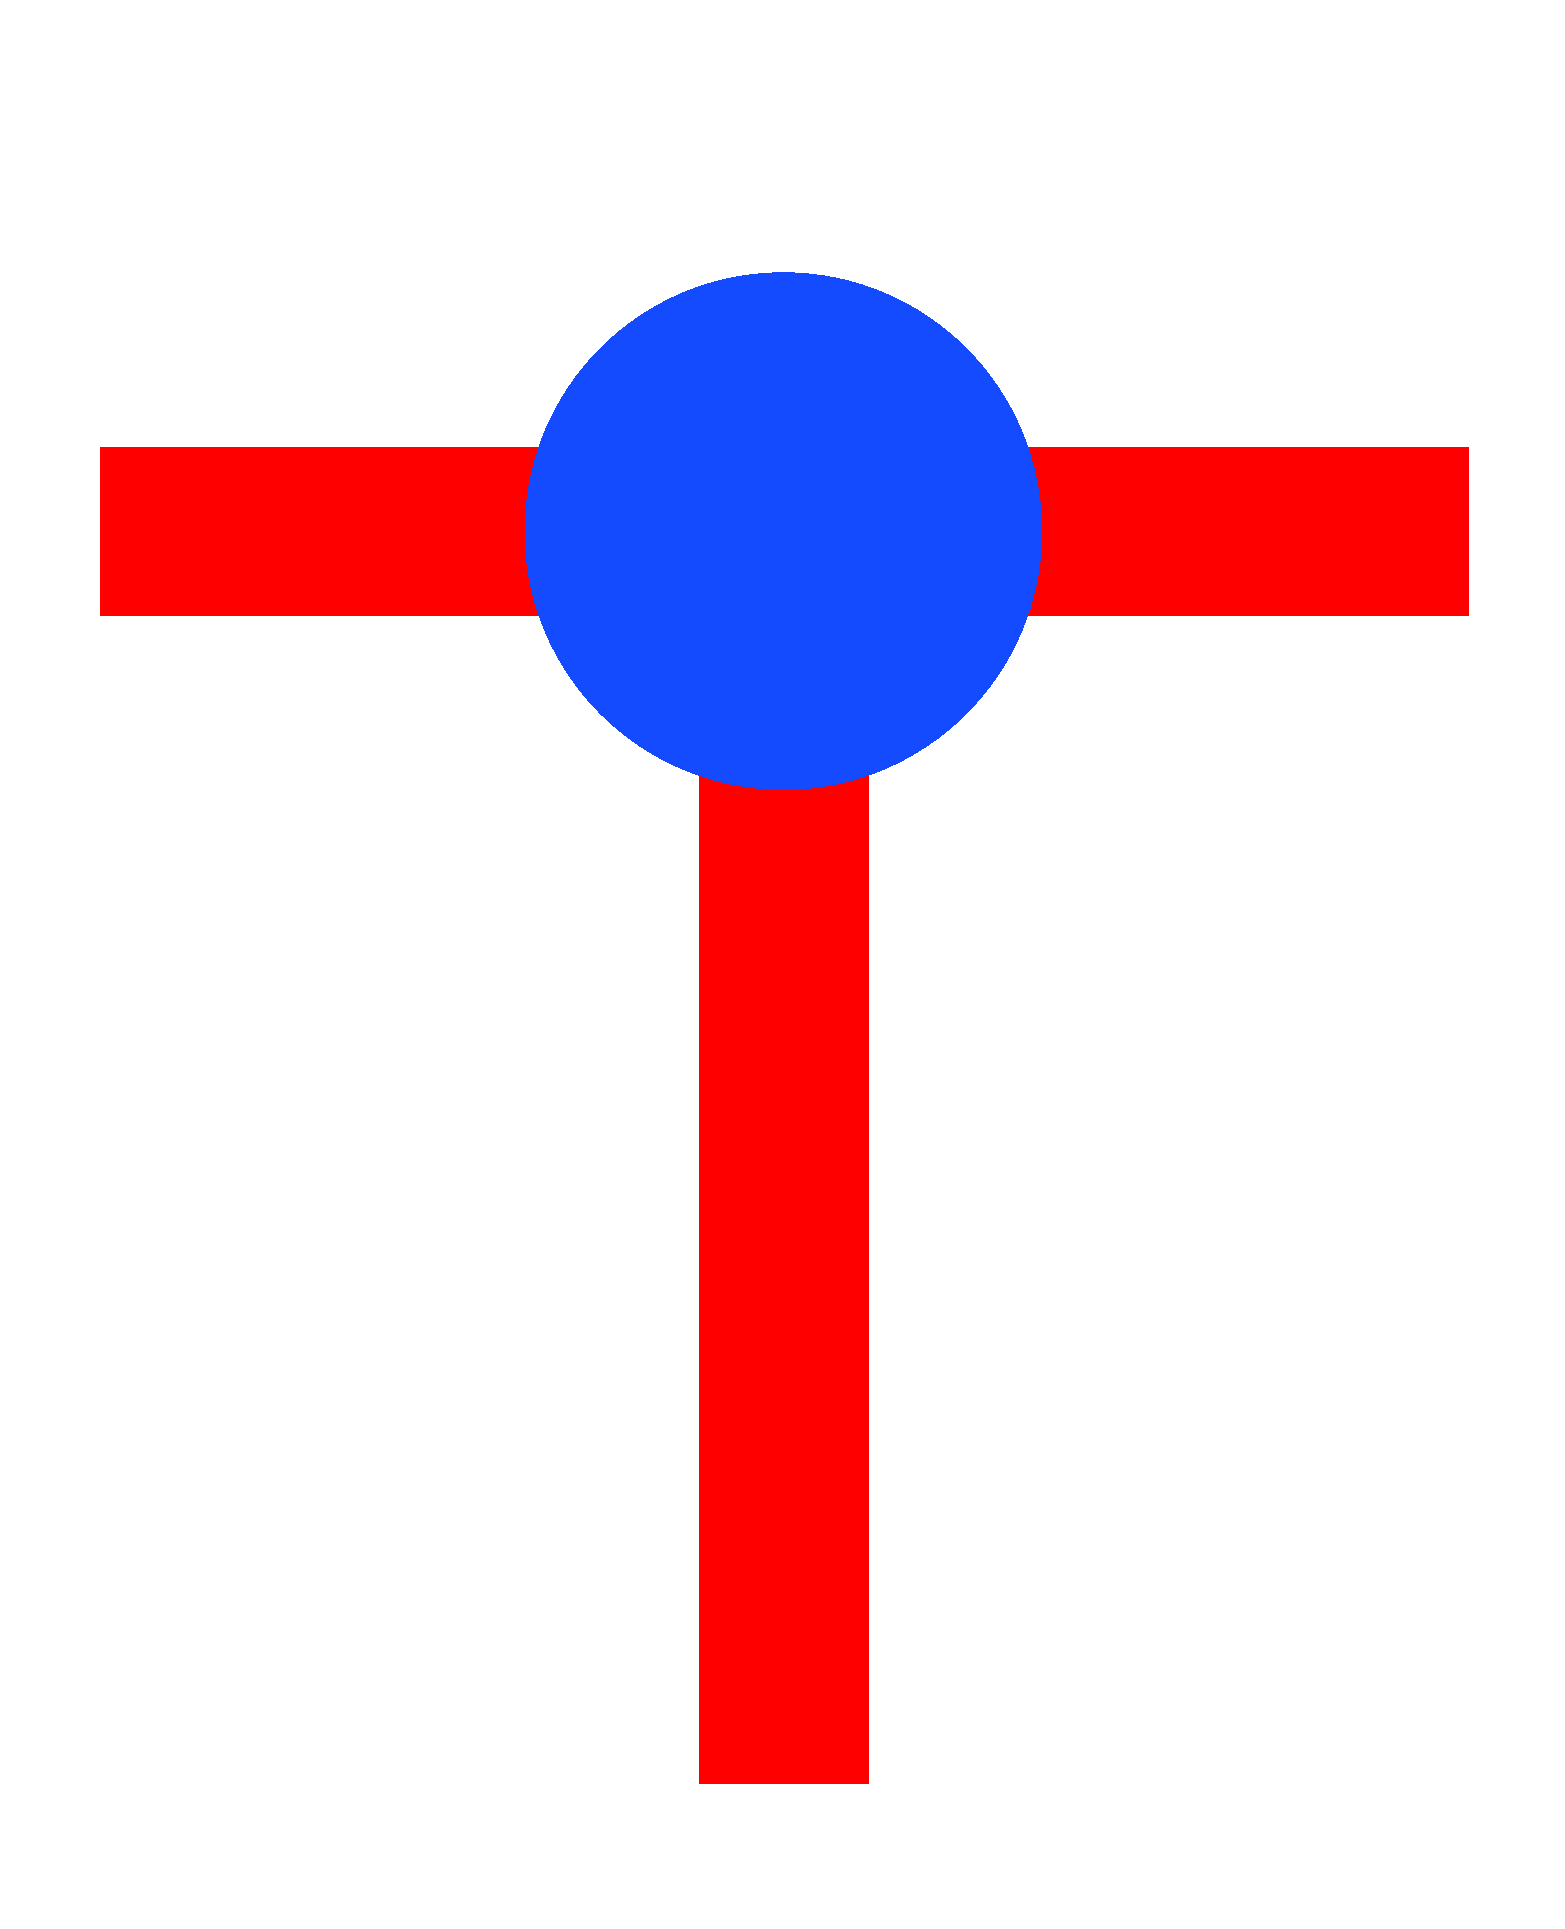
\includegraphics[,height=50mm]{assets/road_shape_T.eps}
        \end{center}
        \caption{T字}
        \label{T}
    \end{minipage}
    \begin{minipage}{0.5\hsize}
        \begin{center}
            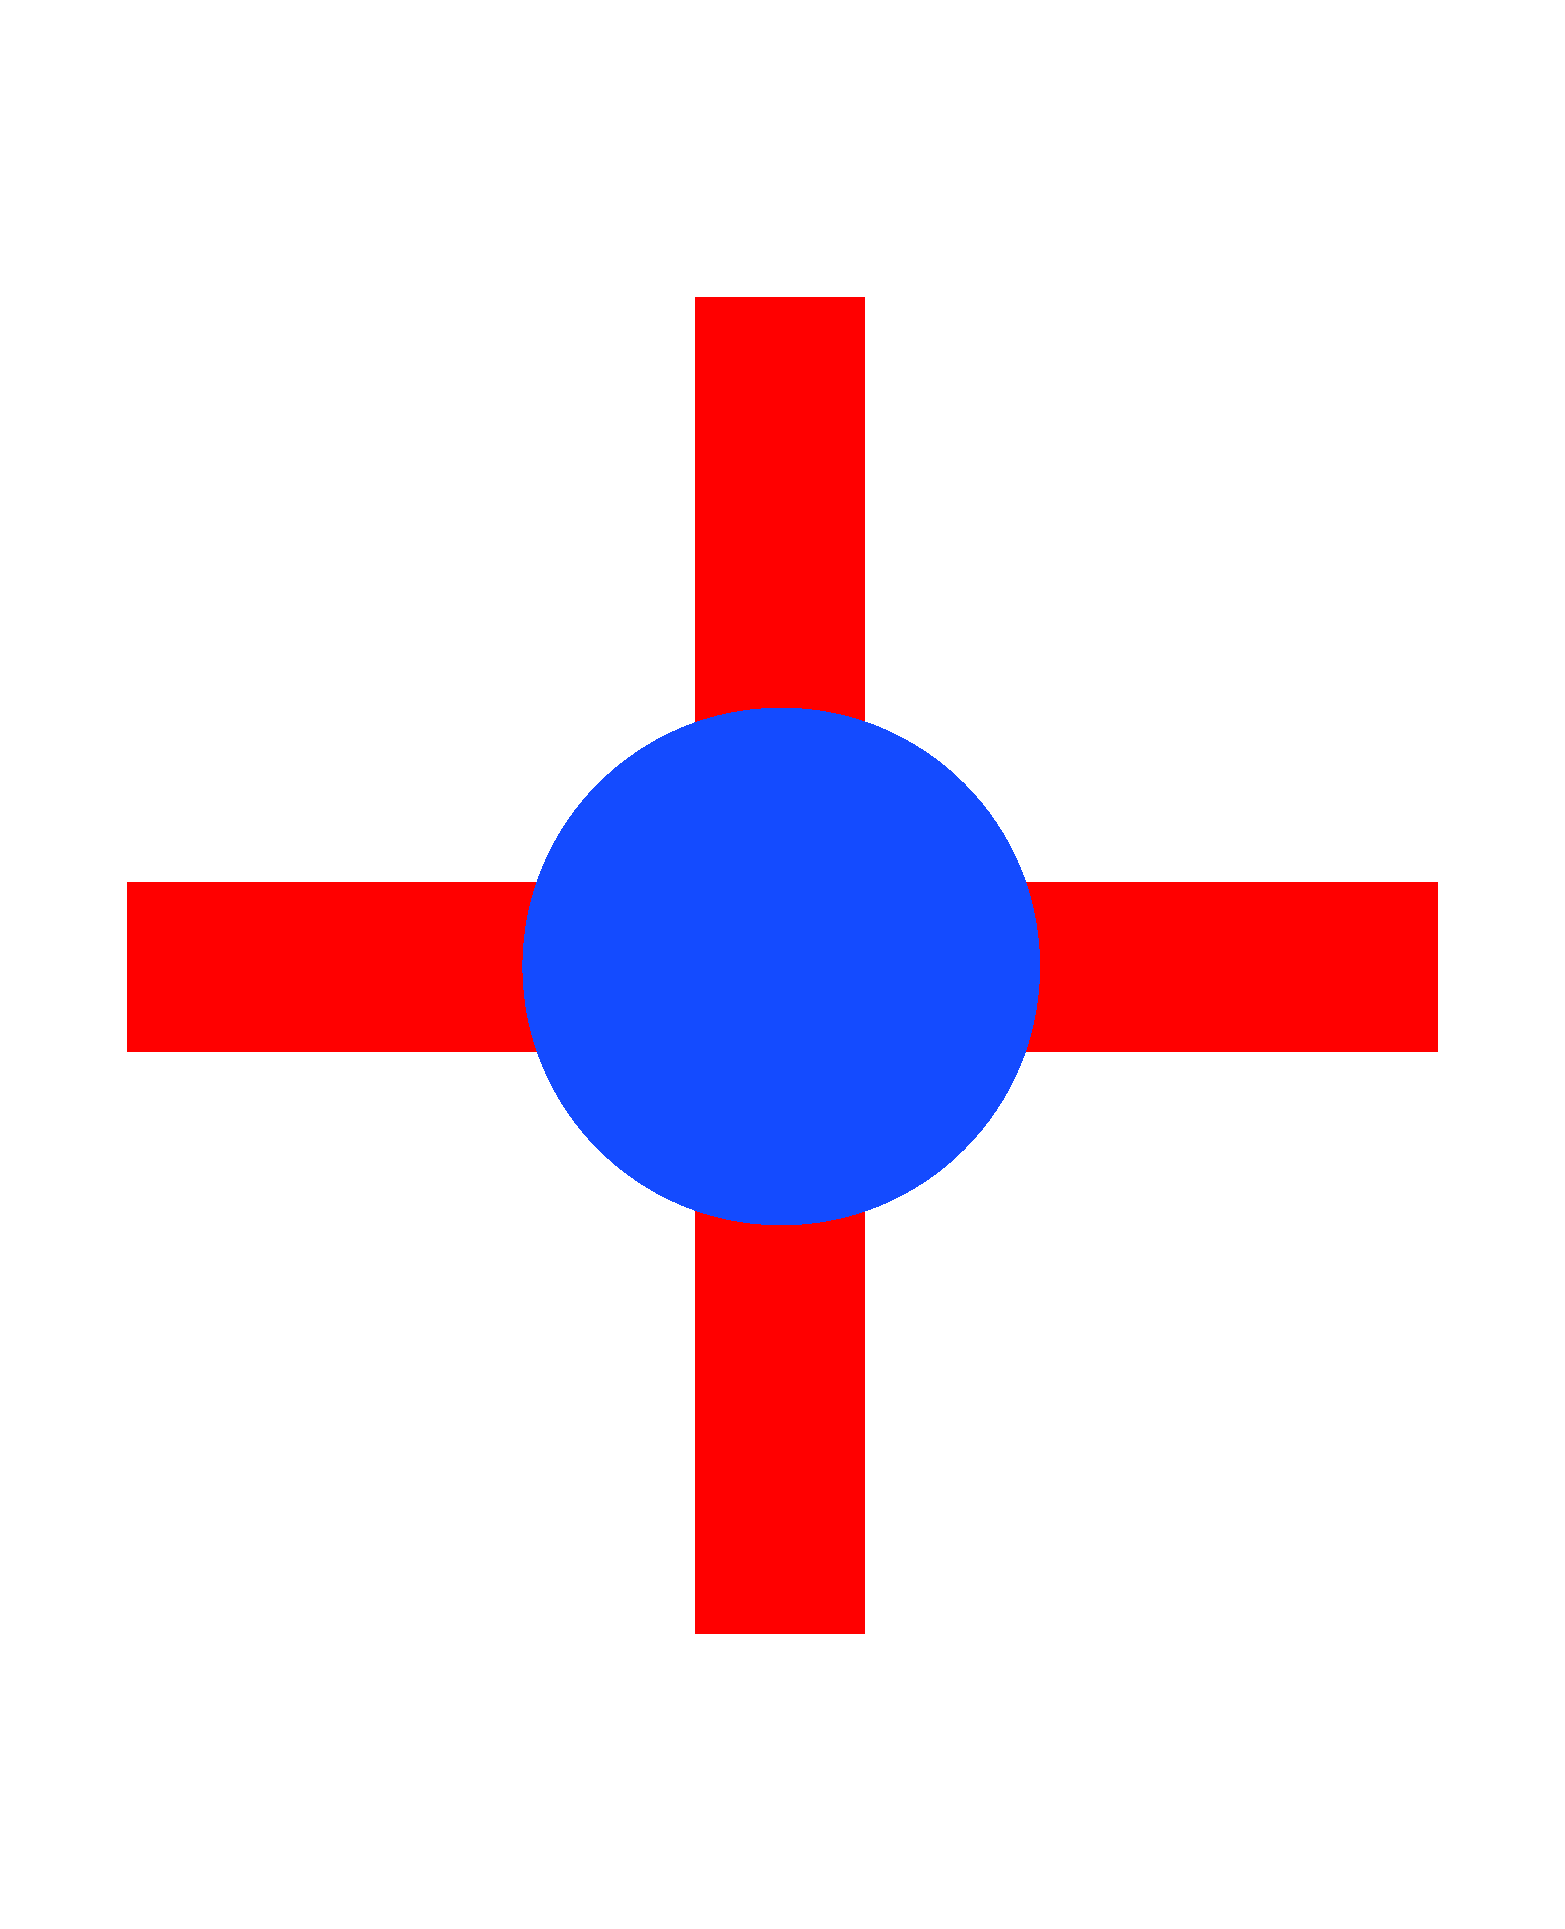
\includegraphics[,height=50mm]{assets/road_shape_Cross.eps}
        \end{center}
        \caption{十字}
        \label{Cross}
    \end{minipage}
\end{figure}




\begin{figure}[htbp]
    \begin{minipage}{0.5\hsize}
        \begin{center}
            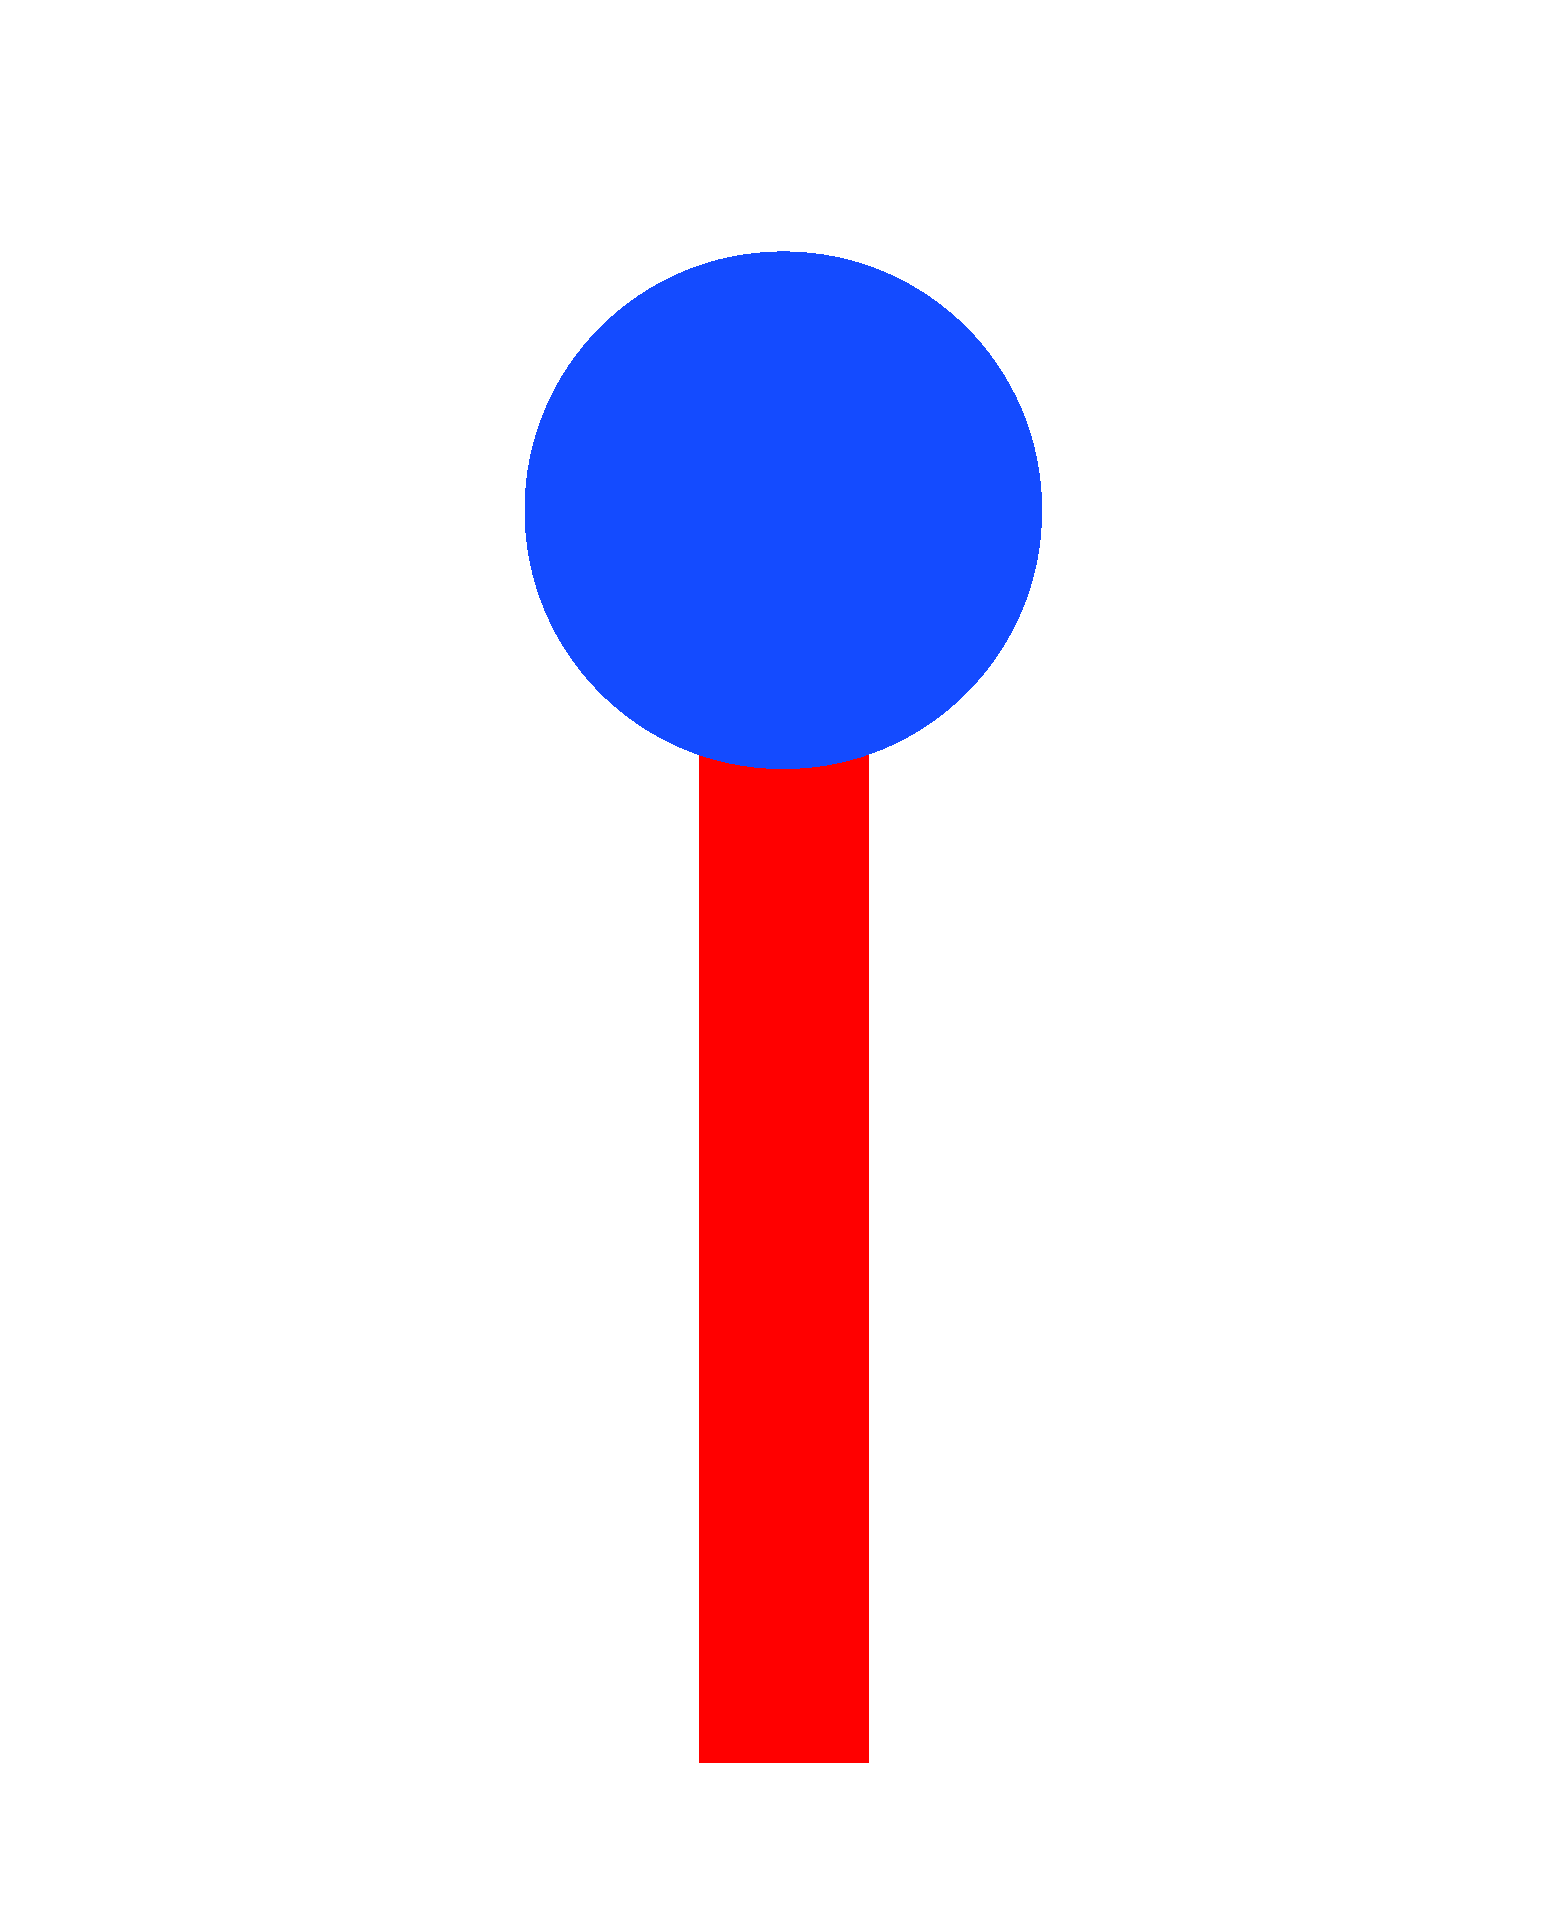
\includegraphics[,height=50mm]{assets/road_shape_End.eps}
        \end{center}
        \caption{行き止まり}
        \label{RouteEnd}
    \end{minipage}
    \begin{minipage}{0.5\hsize}
        \begin{center}
            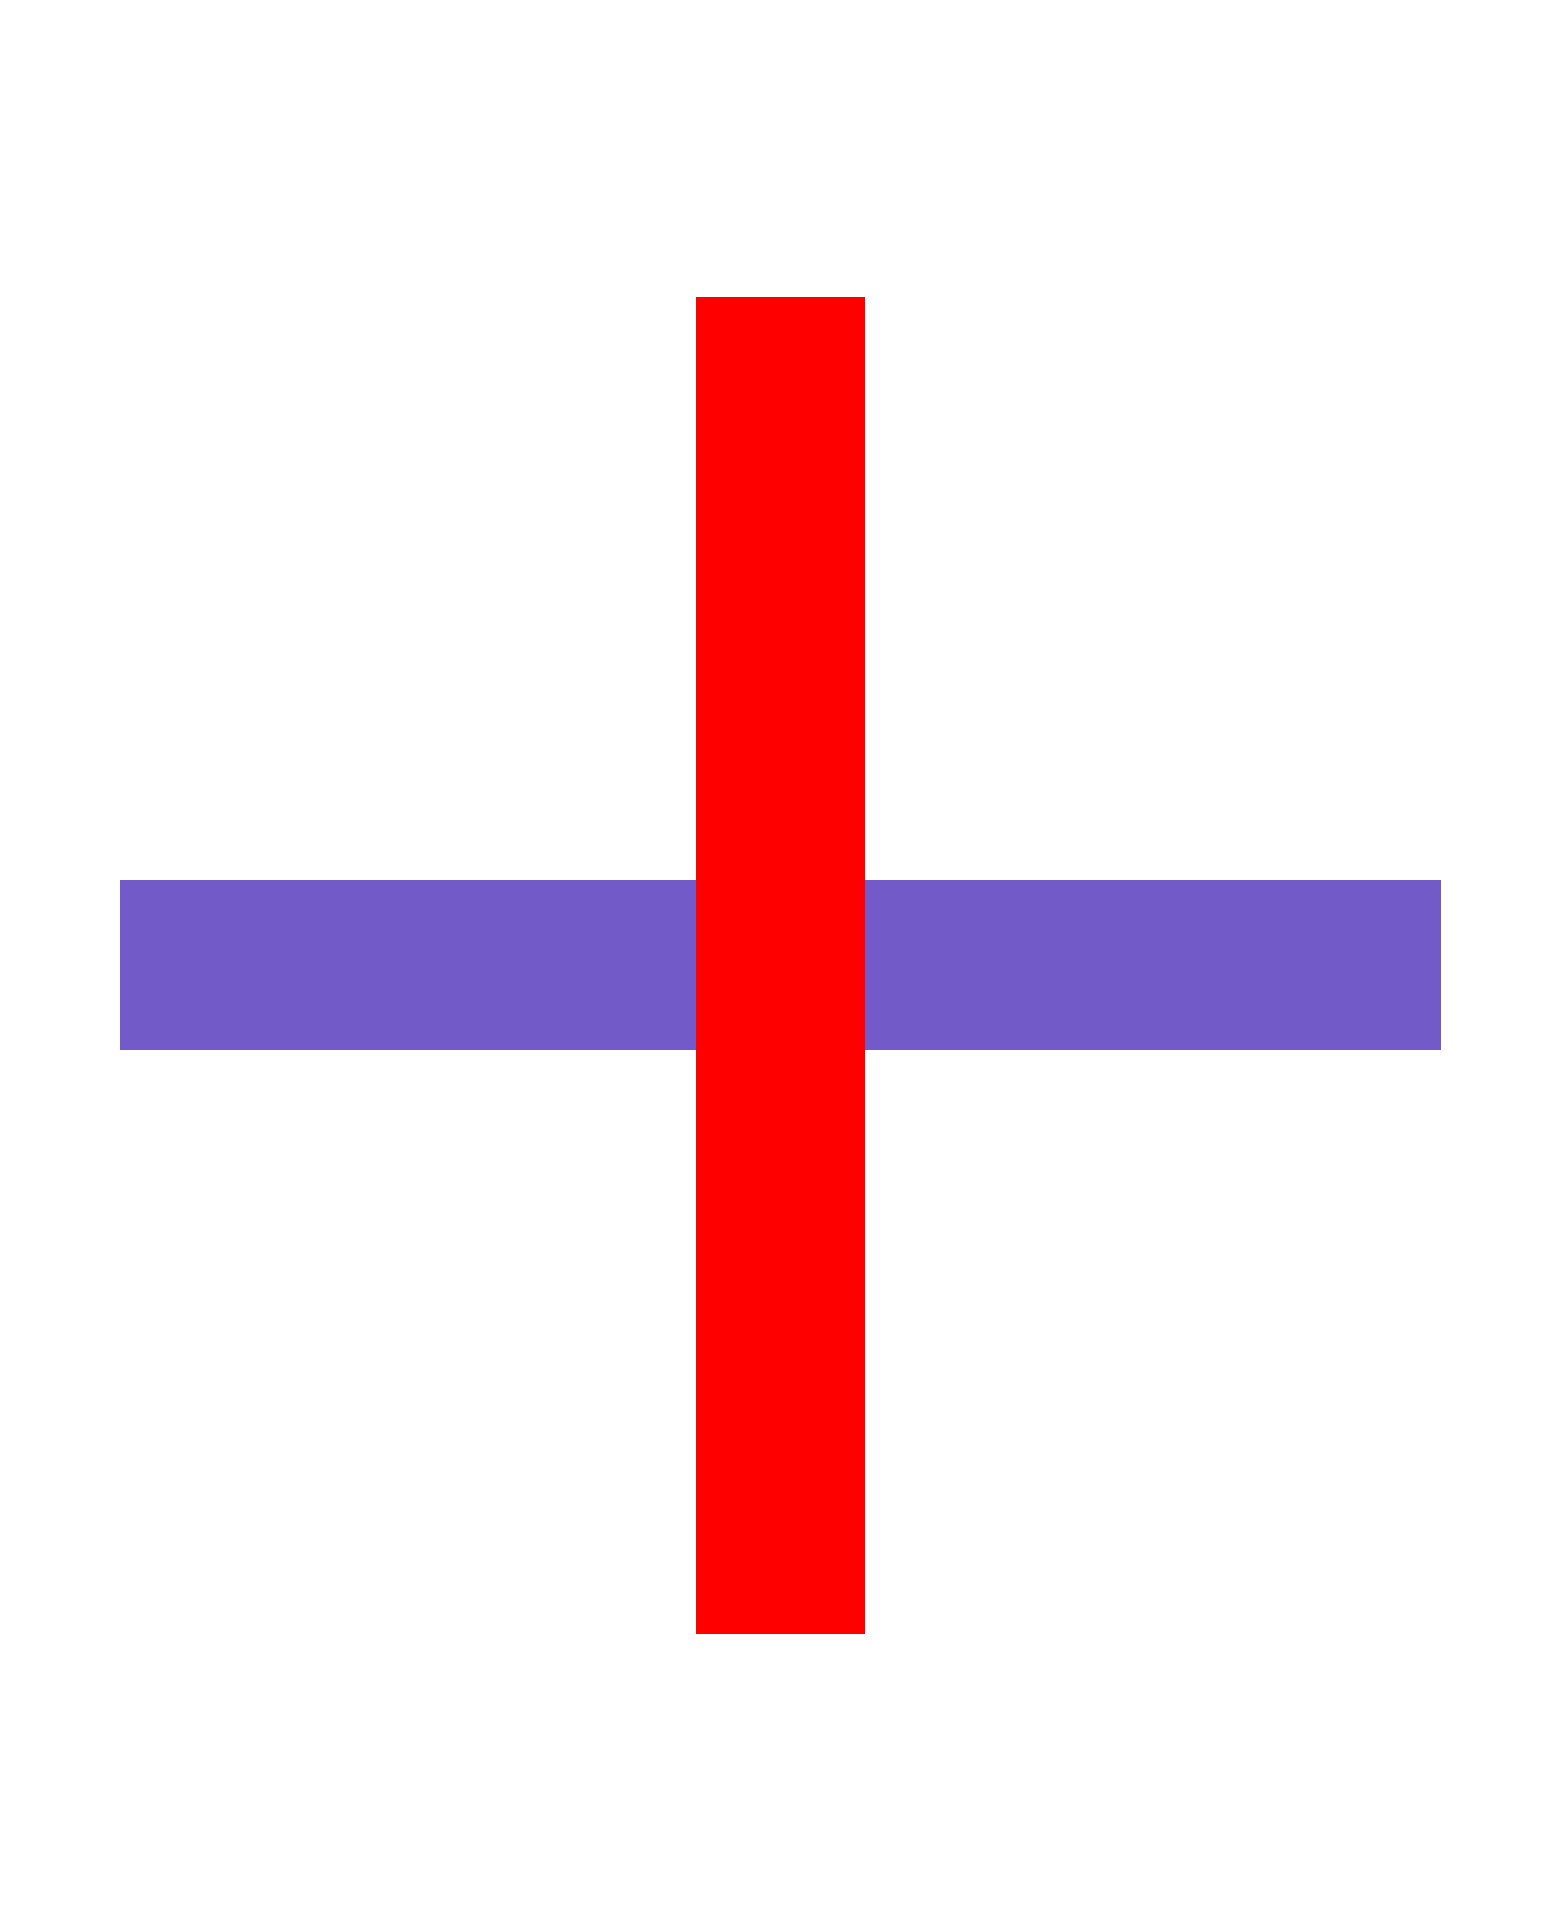
\includegraphics[,height=50mm]{assets/road_shape_GradeSeparation.eps}
        \end{center}
        \caption{立体交差}
        \label{GradeSeparation}
    \end{minipage}
\end{figure}


しかしながら, 上記であげたパターンでは最高4方向への分離飲みしか想定されていない. 従って, 図~\ref{MultipleRoadMerge}のような5線以上が交わるパターンの線形は新たに仮想交差点を追加することにより表現を可能にした.


\begin{figure}[H]
    \centering  % 図を真ん中に配置
    
\includegraphics[clip,width = 13.0cm]{assets/Multiple_Road_Shape.eps}
    \caption{4線以上の道路が1交差地点に合流する場合の変換}  \label{MultipleRoadMerge}
\end{figure}


\section{人間のユースケースの定義}

本研究では以下の利用者のユースケースを想定し, これらの目的を満たせるルートを選択した場合にDQNモデルに対して報酬値を与える環境プログラムを作成した.

\begin{table}[h]
    \caption{実験に利用したユースケース}
    \label{table:SpeedOfLight}
    \centering
    \begin{tabular}{clll}
      \hline
        想定した人 & 状態 \\
        \hline \hline
        自宅へ帰宅する会社員 & 途中で外食を考えている \\
        空港へ急行しなければならない旅行客 & 最短時間で行きたいと考えている \\
        ジュースを飲みたいと思っている人 & 急いではないが, 自販機を利用したい \\
      \hline
    \end{tabular}
  \end{table}
  



\section{DQNモデルによる学習}

DQNモデルによる経路探索を行う. DQNには図~\ref{ll_tensor}のような13x13次元の正方行列を入力する.


\begin{figure}[H]
    \centering  % 図を真ん中に配置
    \includegraphics[clip,width = 11.0cm]{assets/MAP_6.eps}
    \caption{入力する正方行列の例} \label{ll_tensor}
\end{figure}
  

\subsection{環境}

エージェントが活動する環境を定義する.

\textcolor{red}{ここに環境定義に関する詳しい説明}

%%% Local Variables:
%%% mode: japanese-latex
%%% TeX-master: "../bthesis"
%%% End:
